\chapter{Regression problem}
\label{app:regression-problem} 

Unless it is specified otherwise, the miscoverage level was set to $\a=0.2$ (\textit{i.e.} $80\%$ of expected coverage) for the visualizations.

\begin{figure}[ht]
    \centering
    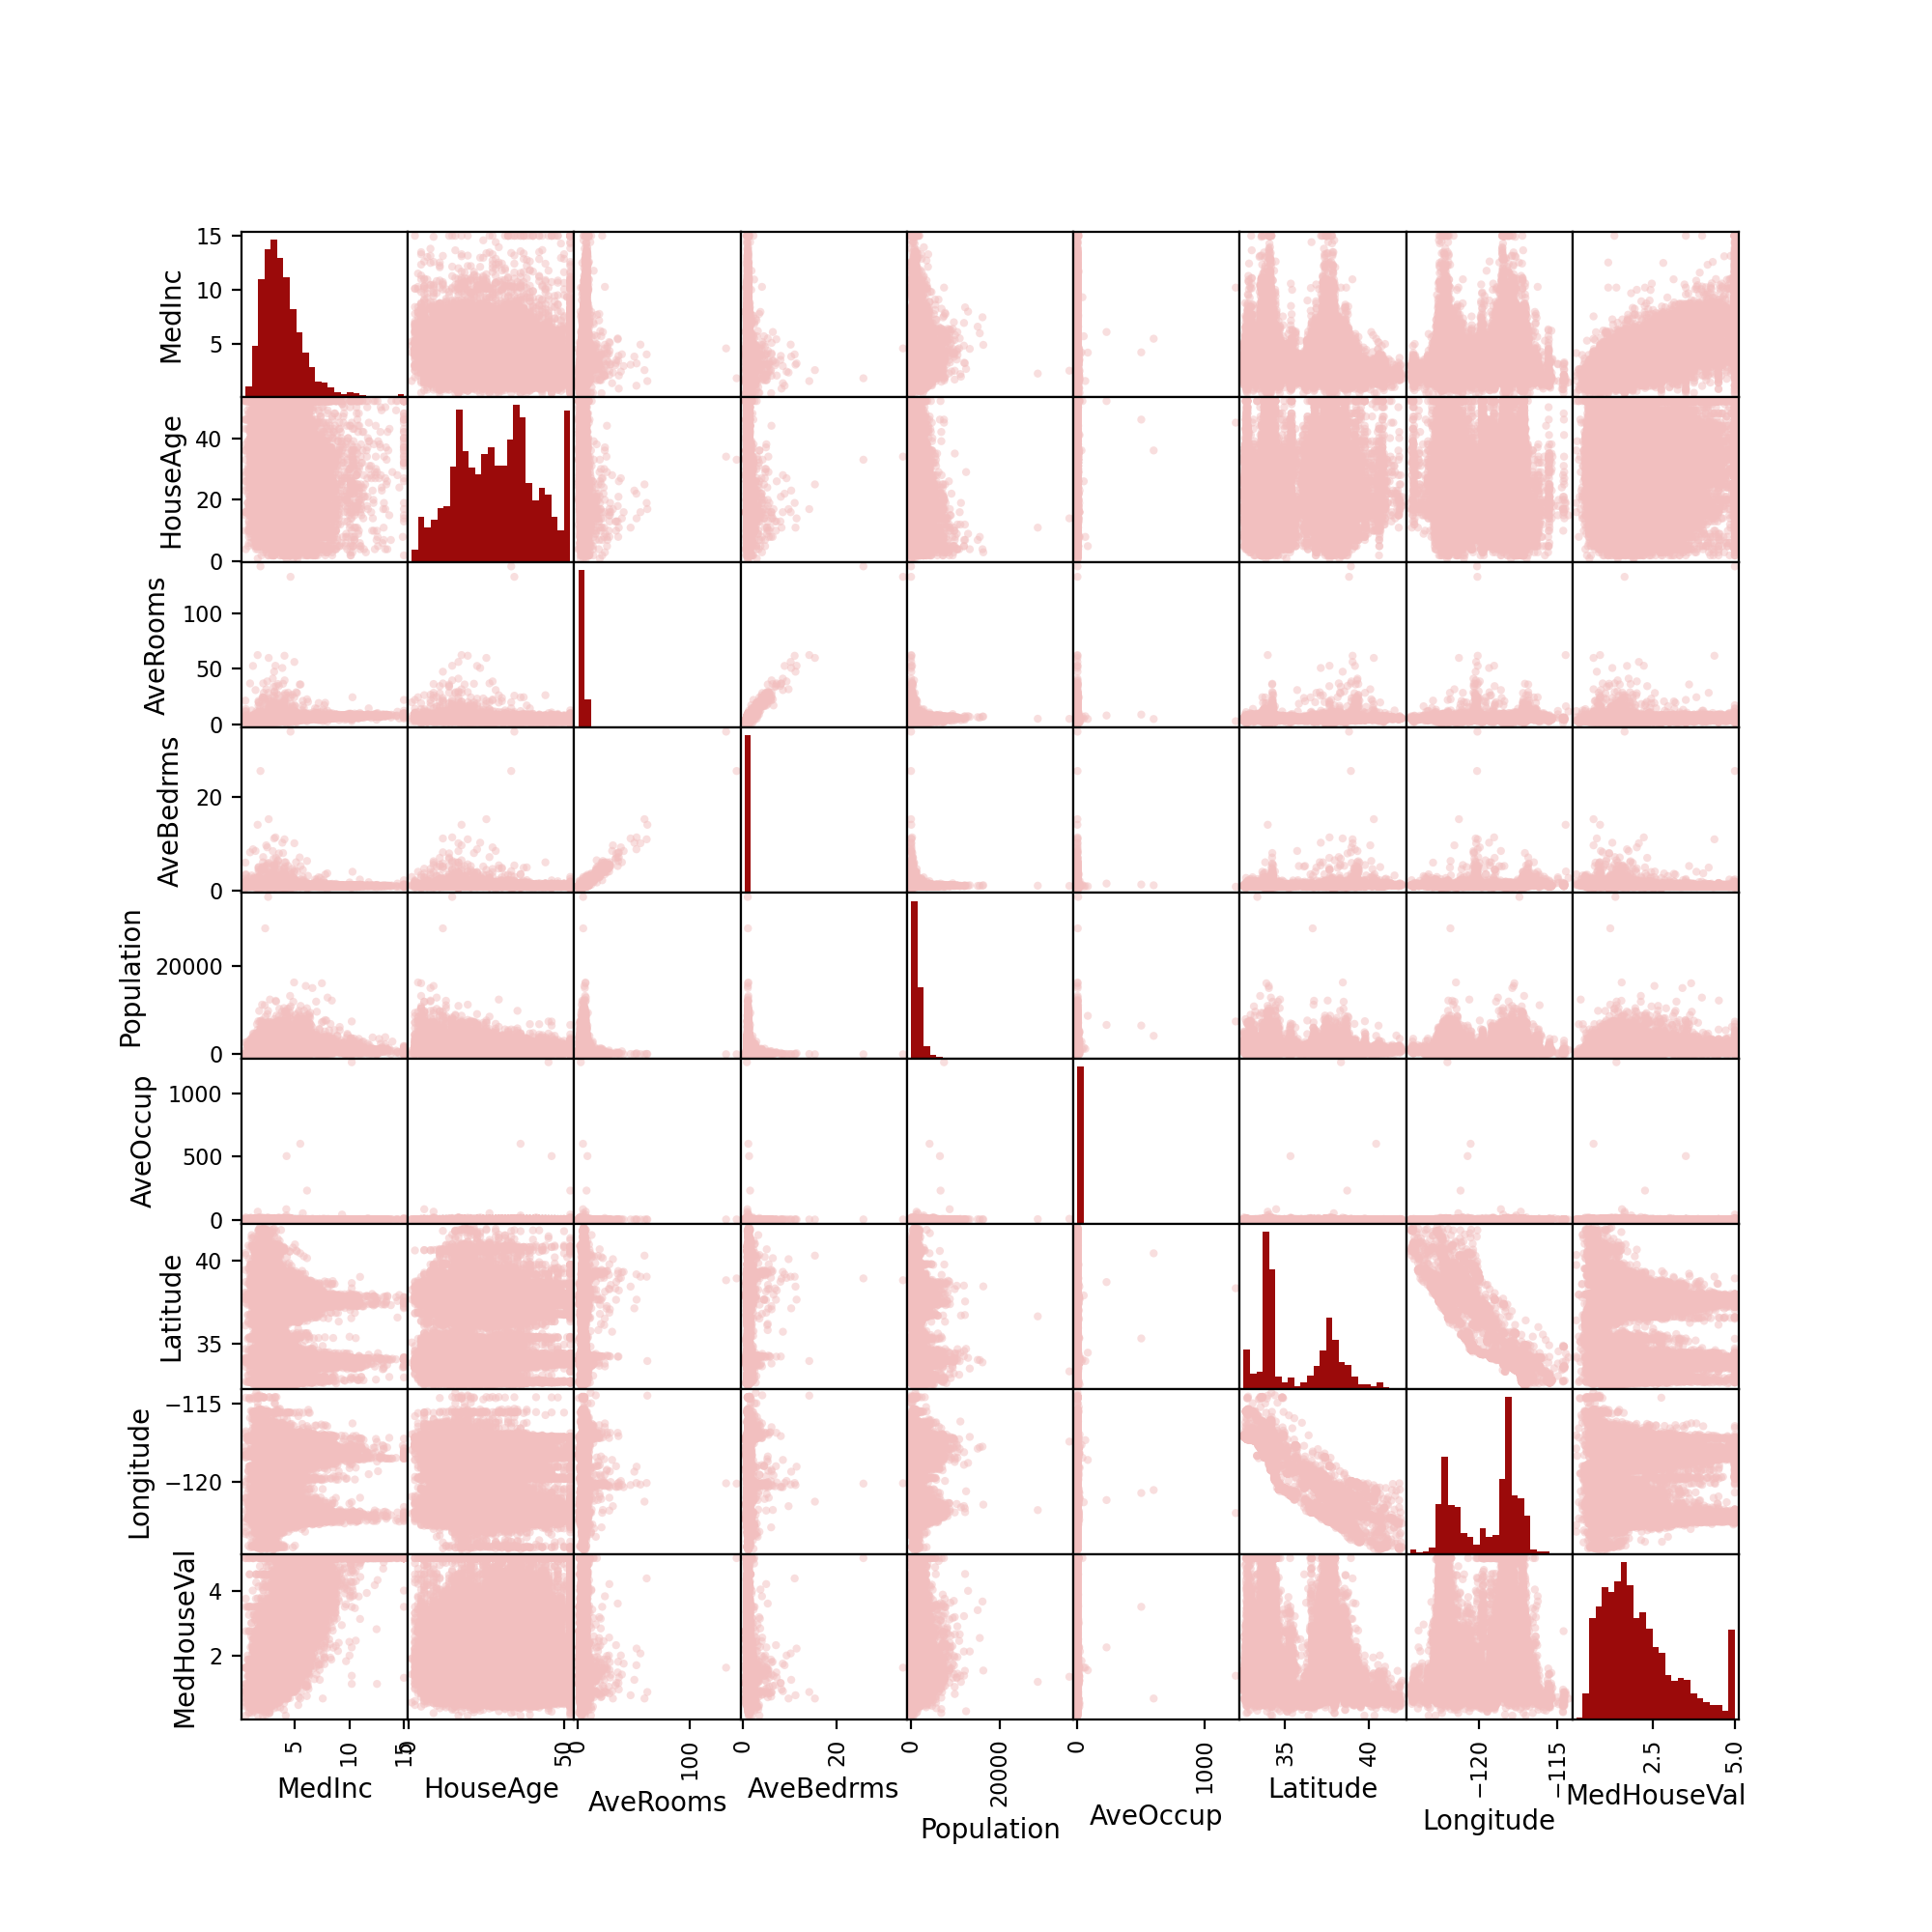
\includegraphics[width=0.8\textwidth]{Figures/regression/data-regression-problem.png}
    \caption{Marginal distributions for each of the possible combinations of the regression problem's features.}
    \label{fig:app-regression-data-distribution}
\end{figure}

\begin{figure}[ht]
    \centering
    \hspace{-10mm}
    \begin{subfigure}[b]{0.48\textwidth}
        \centering
        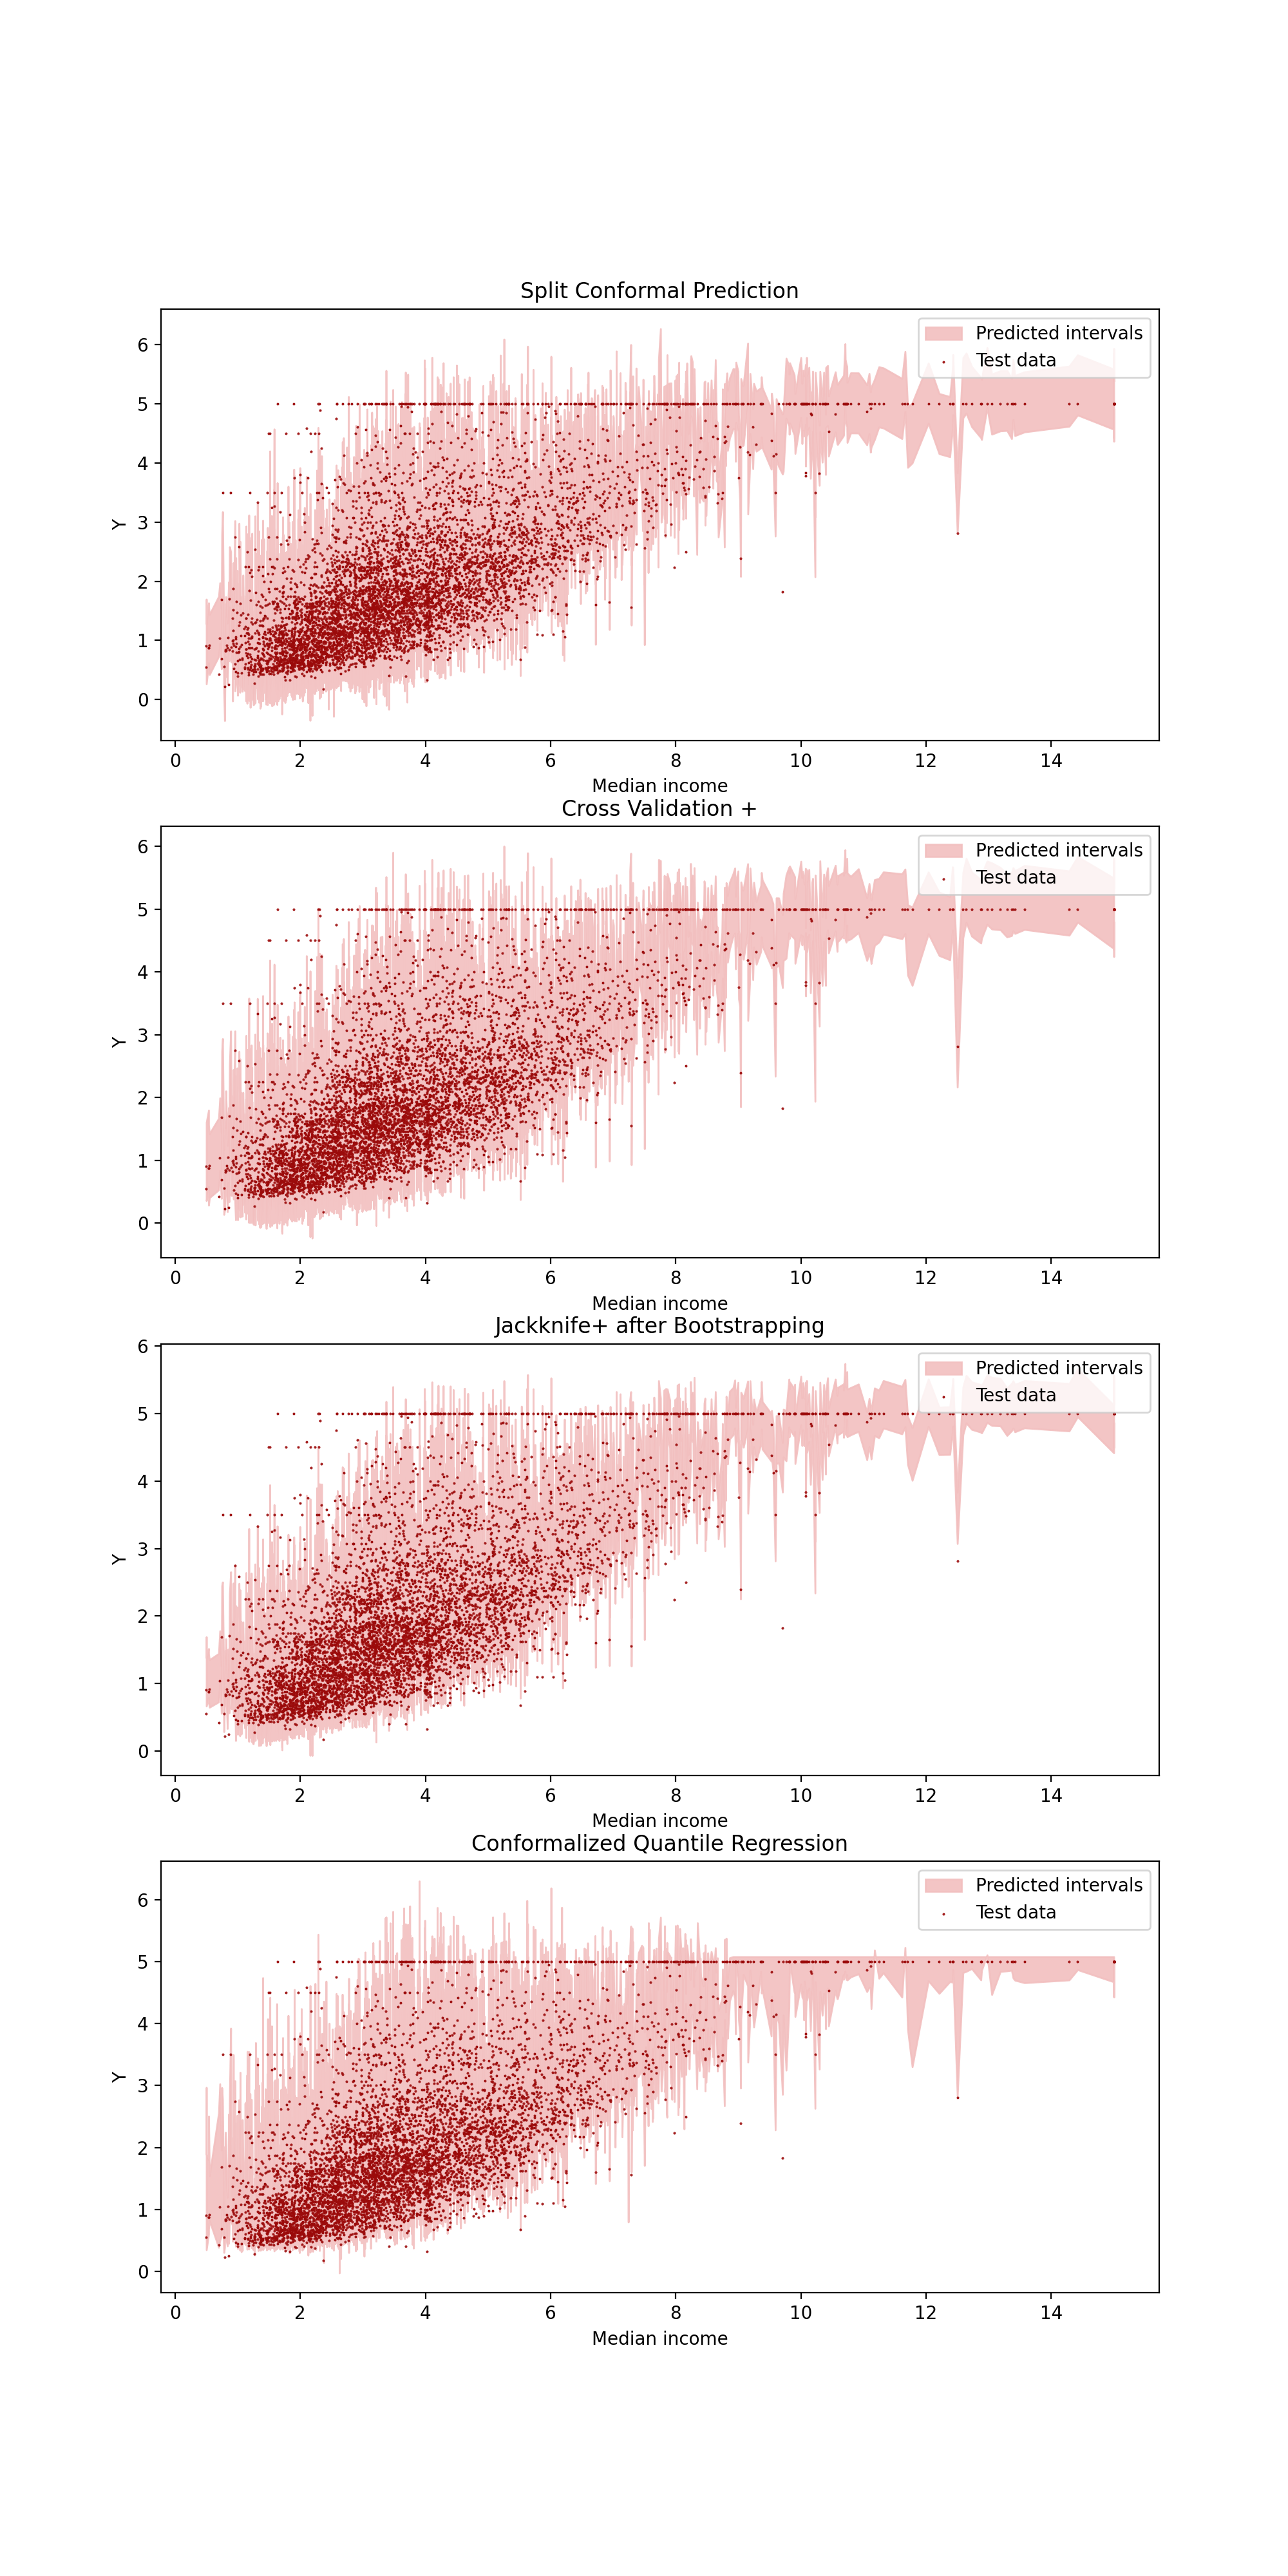
\includegraphics[width=1.2\textwidth, height=3.35\textwidth]{Figures/regression/prediction-intervals-regression-problem.png}
        \caption{Prediction intervals}
        \label{subfig:app-regression-prediction-intervals}
    \end{subfigure}
    \hfill % adds horizontal space between figures
    \begin{subfigure}[b]{0.48\textwidth} % Adjust the width to fit your needs
        \centering
        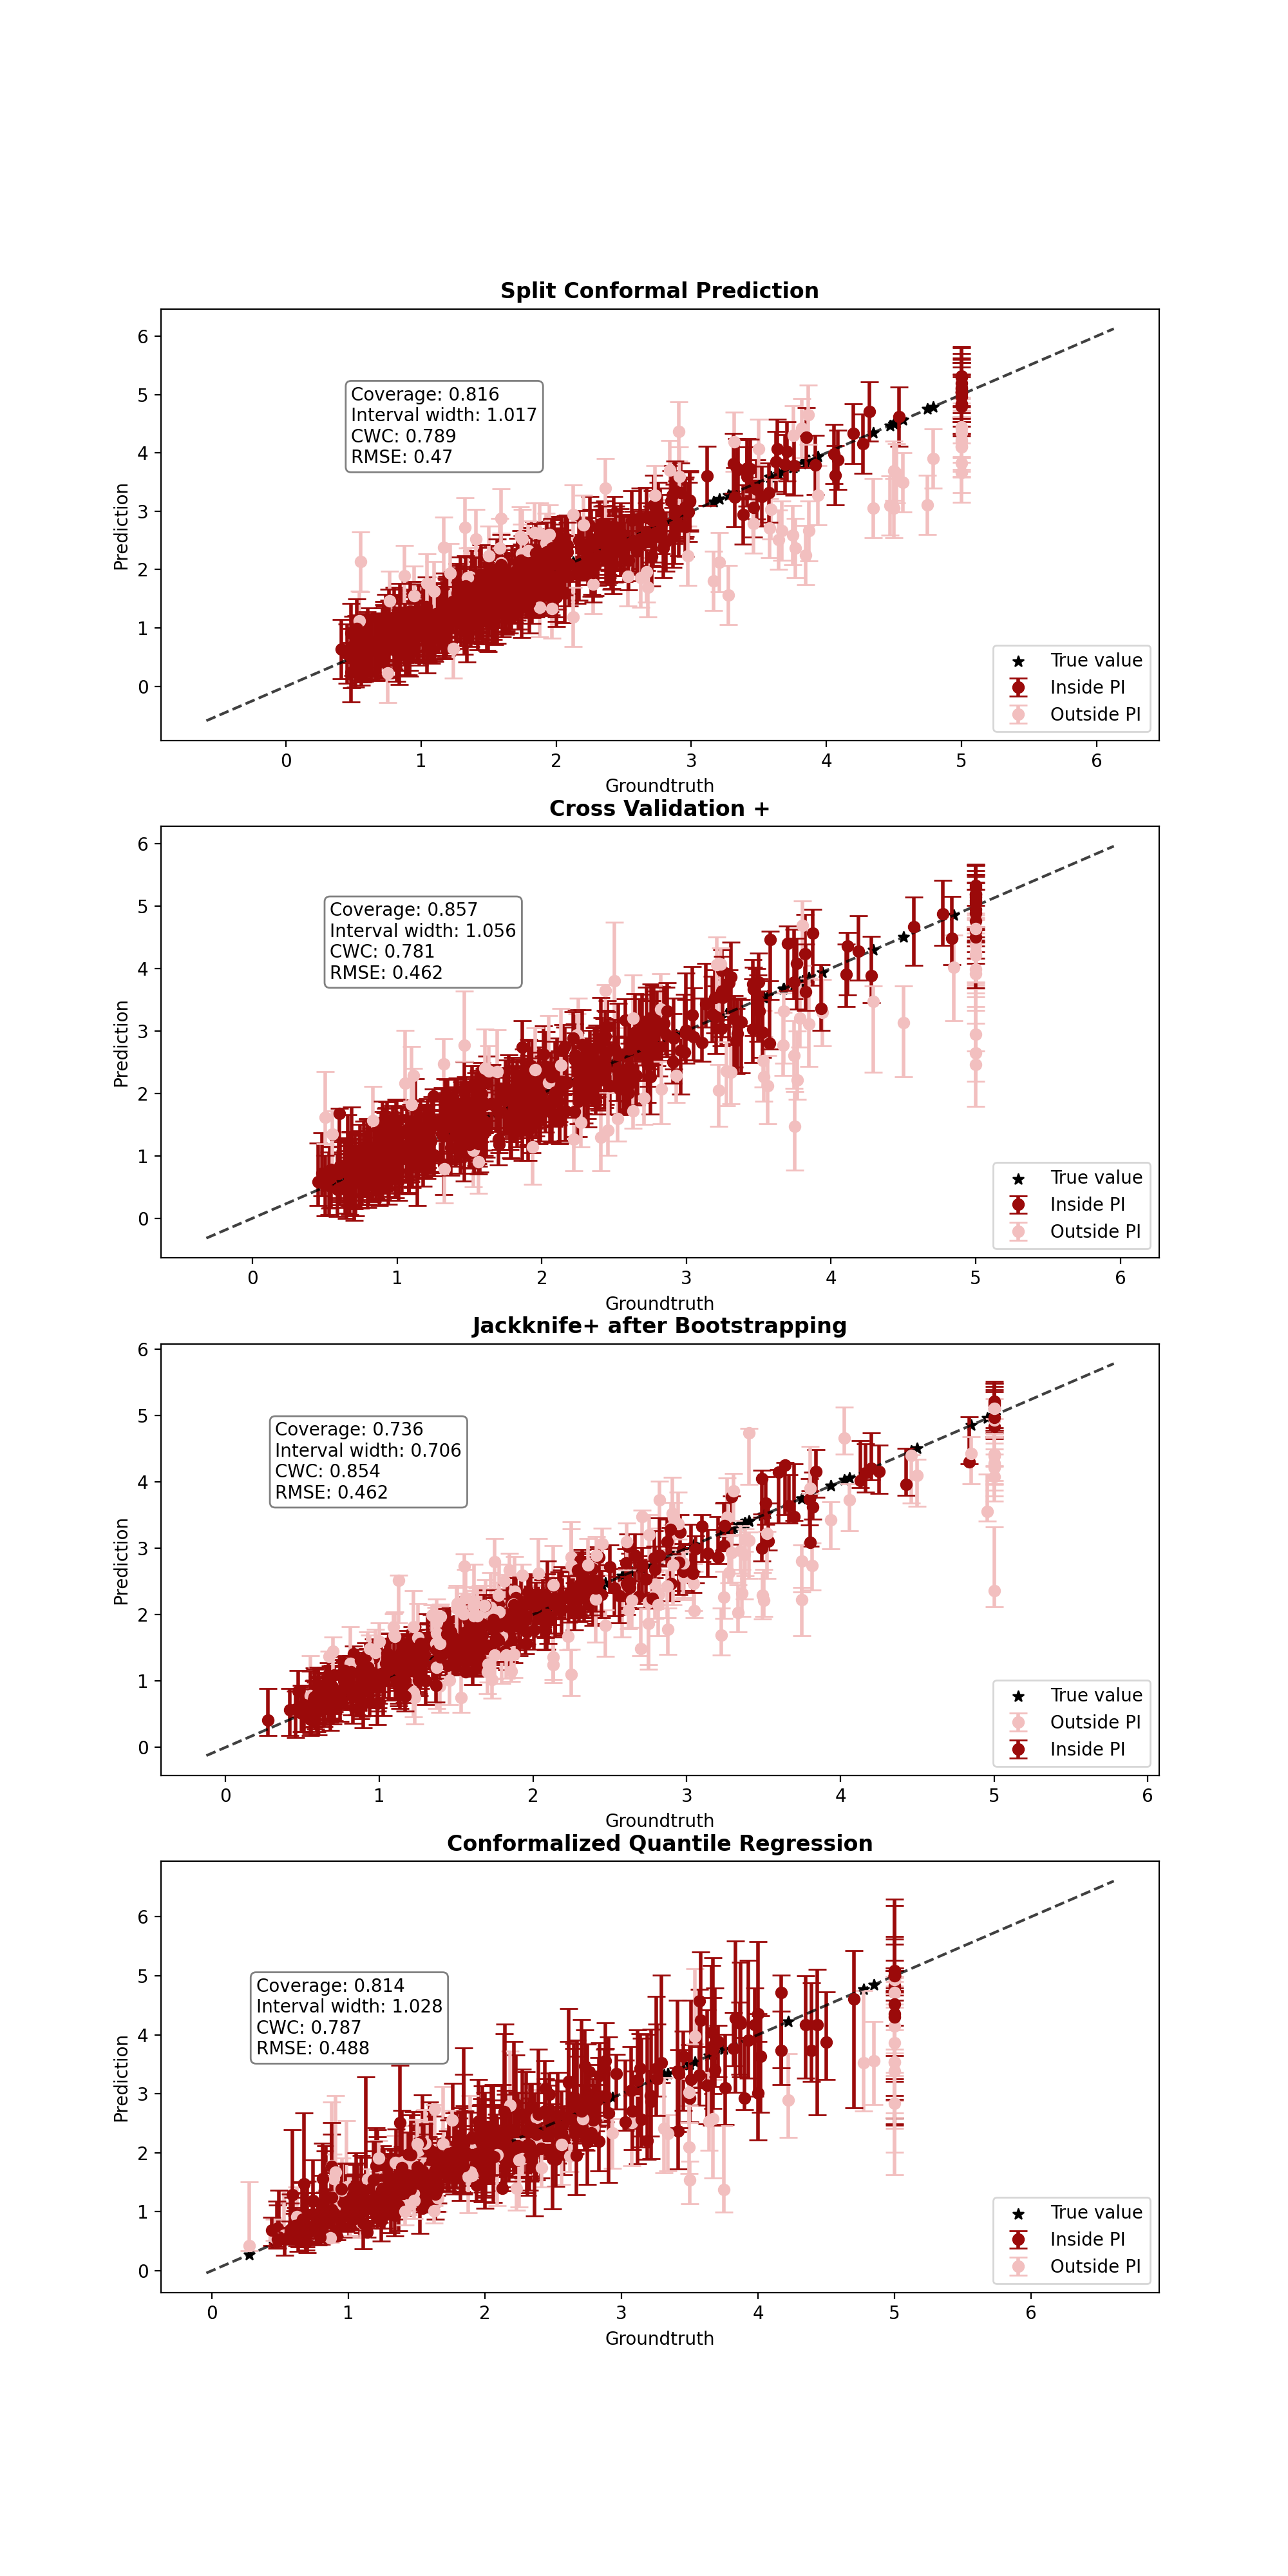
\includegraphics[width=1.2\textwidth, height=3.35\textwidth]{Figures/regression/average-goodness-regression-problem.png} % Adjust the filename and path
        \caption{Goodness of the prediction intervals (prediction vs. ground truth). Just $7.5\%$ was used for visualization purposes.}
        \label{subfig:app-regression-intervals-goodness}
    \end{subfigure}
    \caption{Visualizations related to the prediction intervals for the test data and 4 different strategies, from top to bottom: SCP, CV$+$, J$+$aB and CQR.}
    \label{fig:app-regression-intervals}
\end{figure}

\begin{figure}[ht]
    \centering
    %\hspace{-10mm}
    \begin{subfigure}[b]{0.32\textwidth}
        \centering
        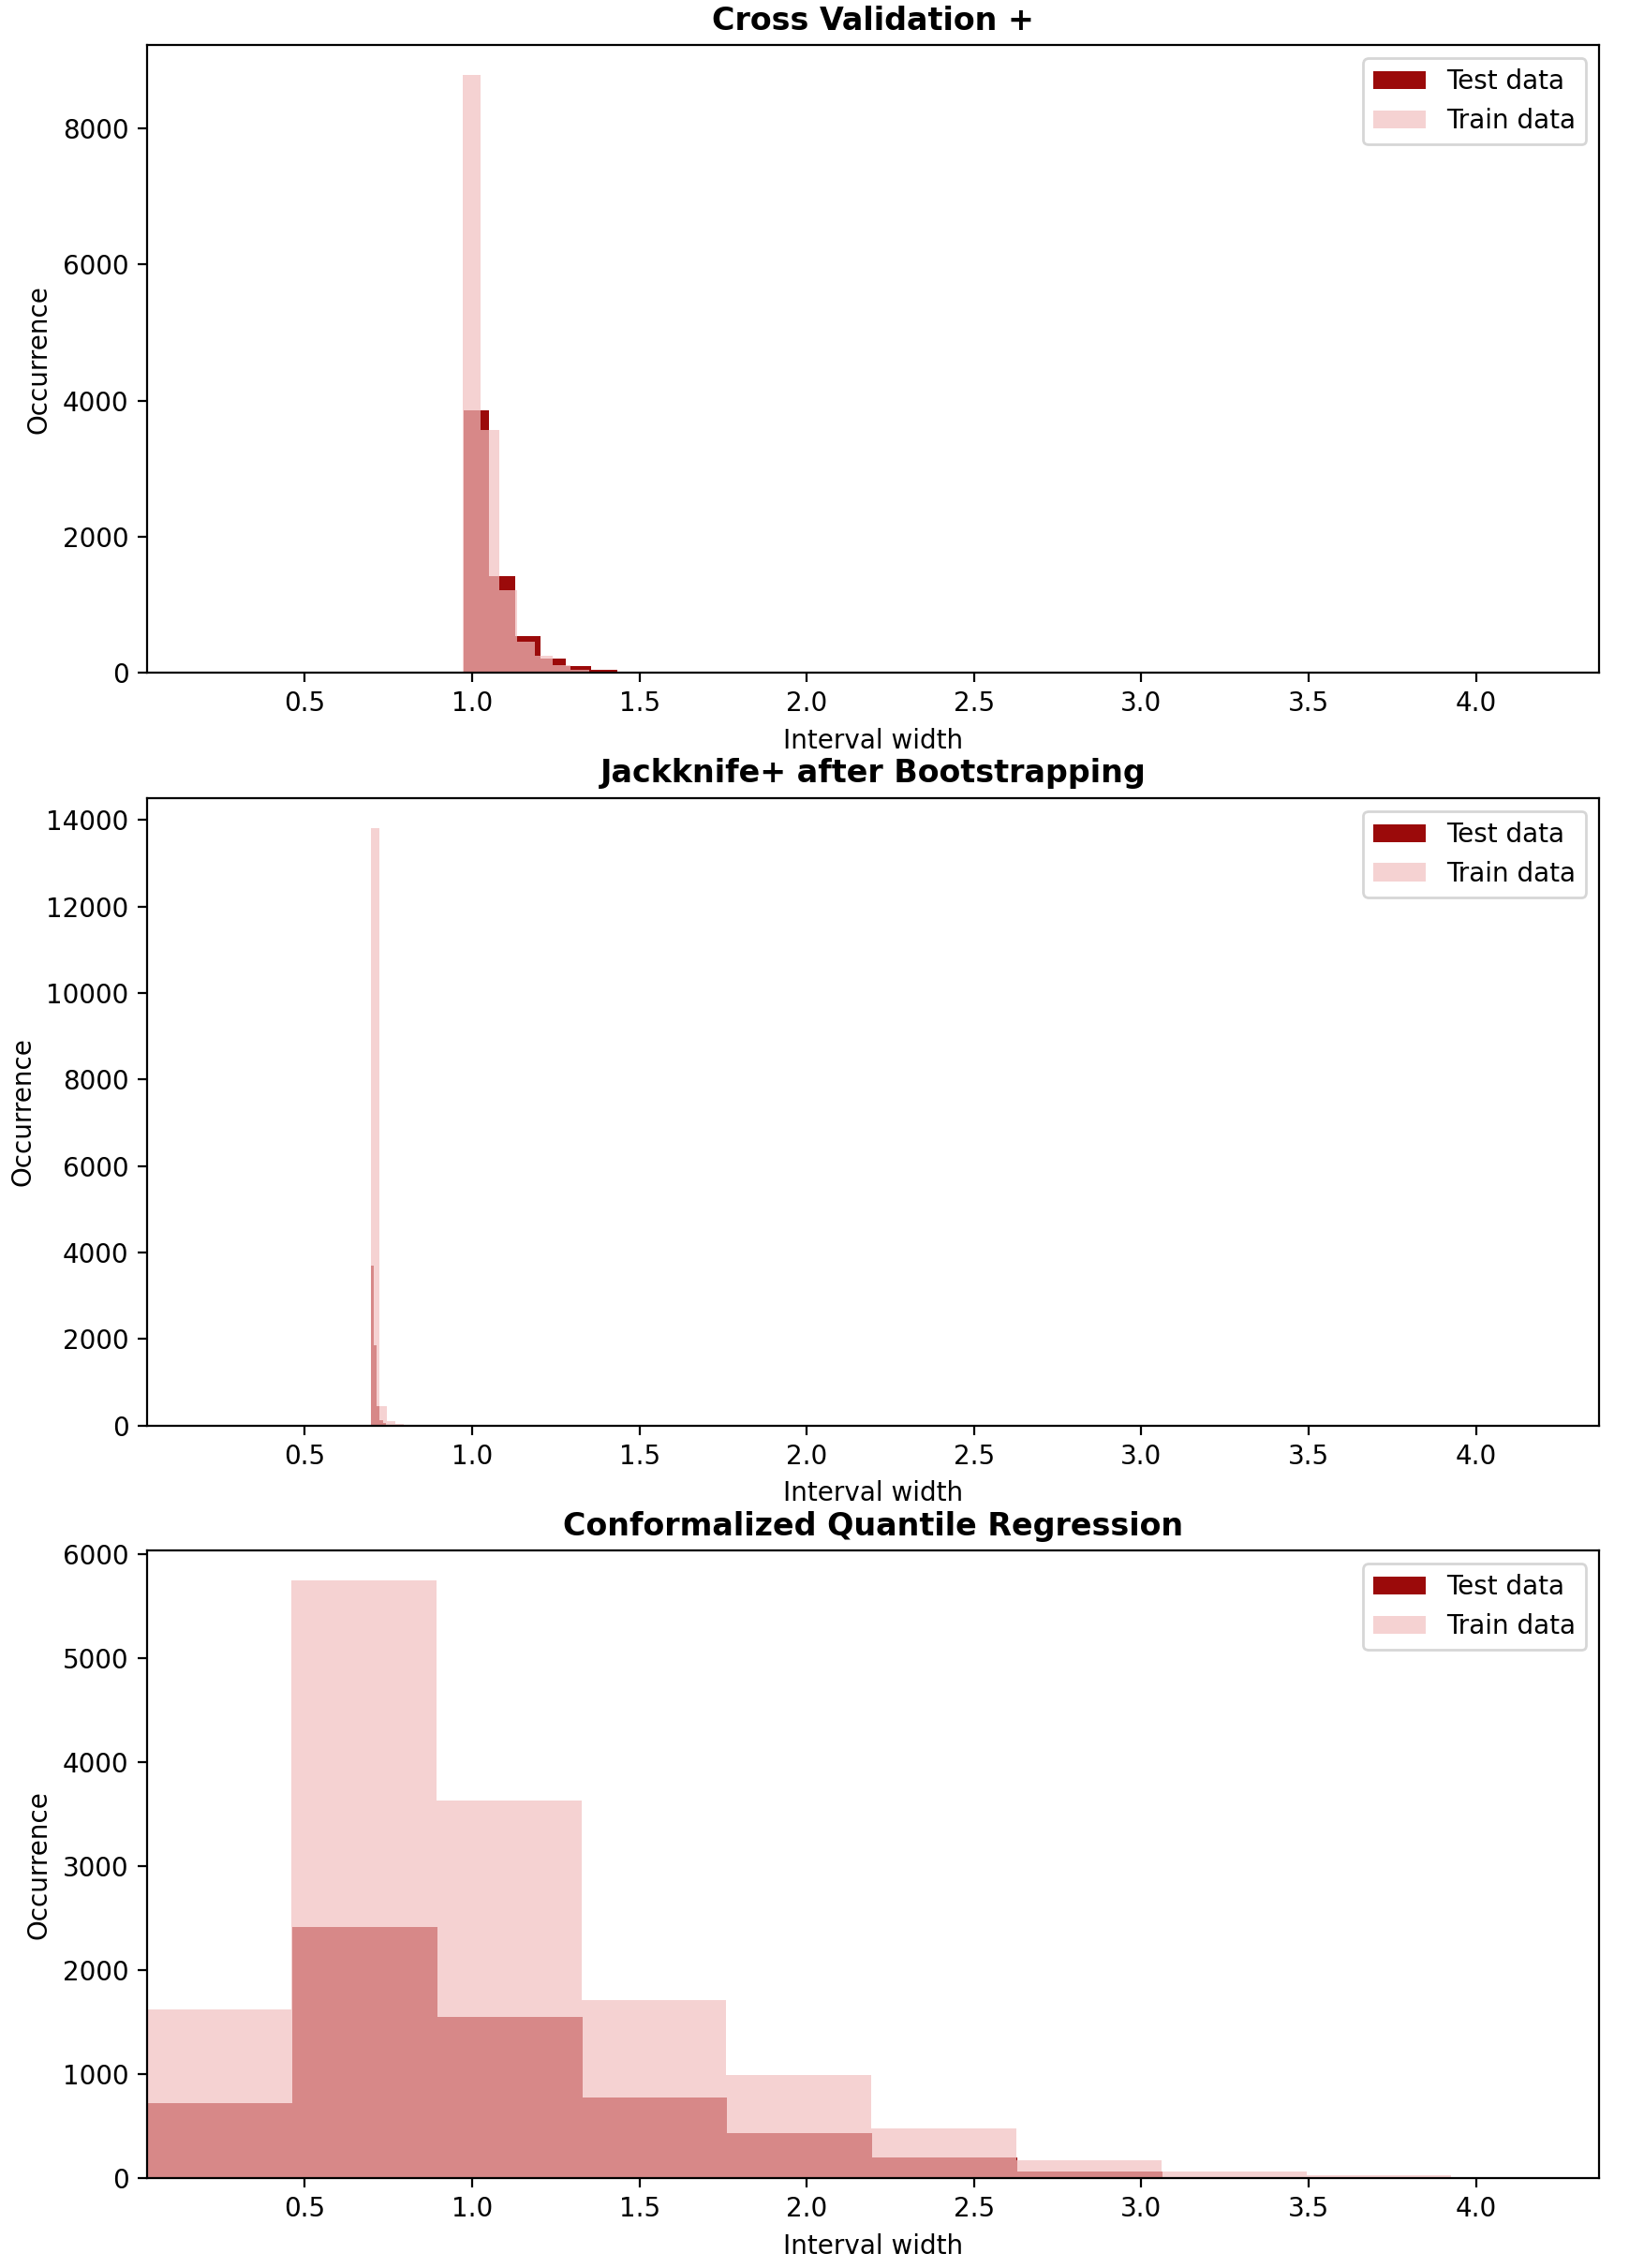
\includegraphics[width=1.15\textwidth, height=3.05\textwidth]{Figures/regression/width-occurrence-regression-problem.png}
        \caption{Intervals' width histograms}
        \label{subfig:app-regression-width-histograms}
    \end{subfigure}
    \hfill
    \begin{subfigure}[b]{0.32\textwidth}
        \centering
        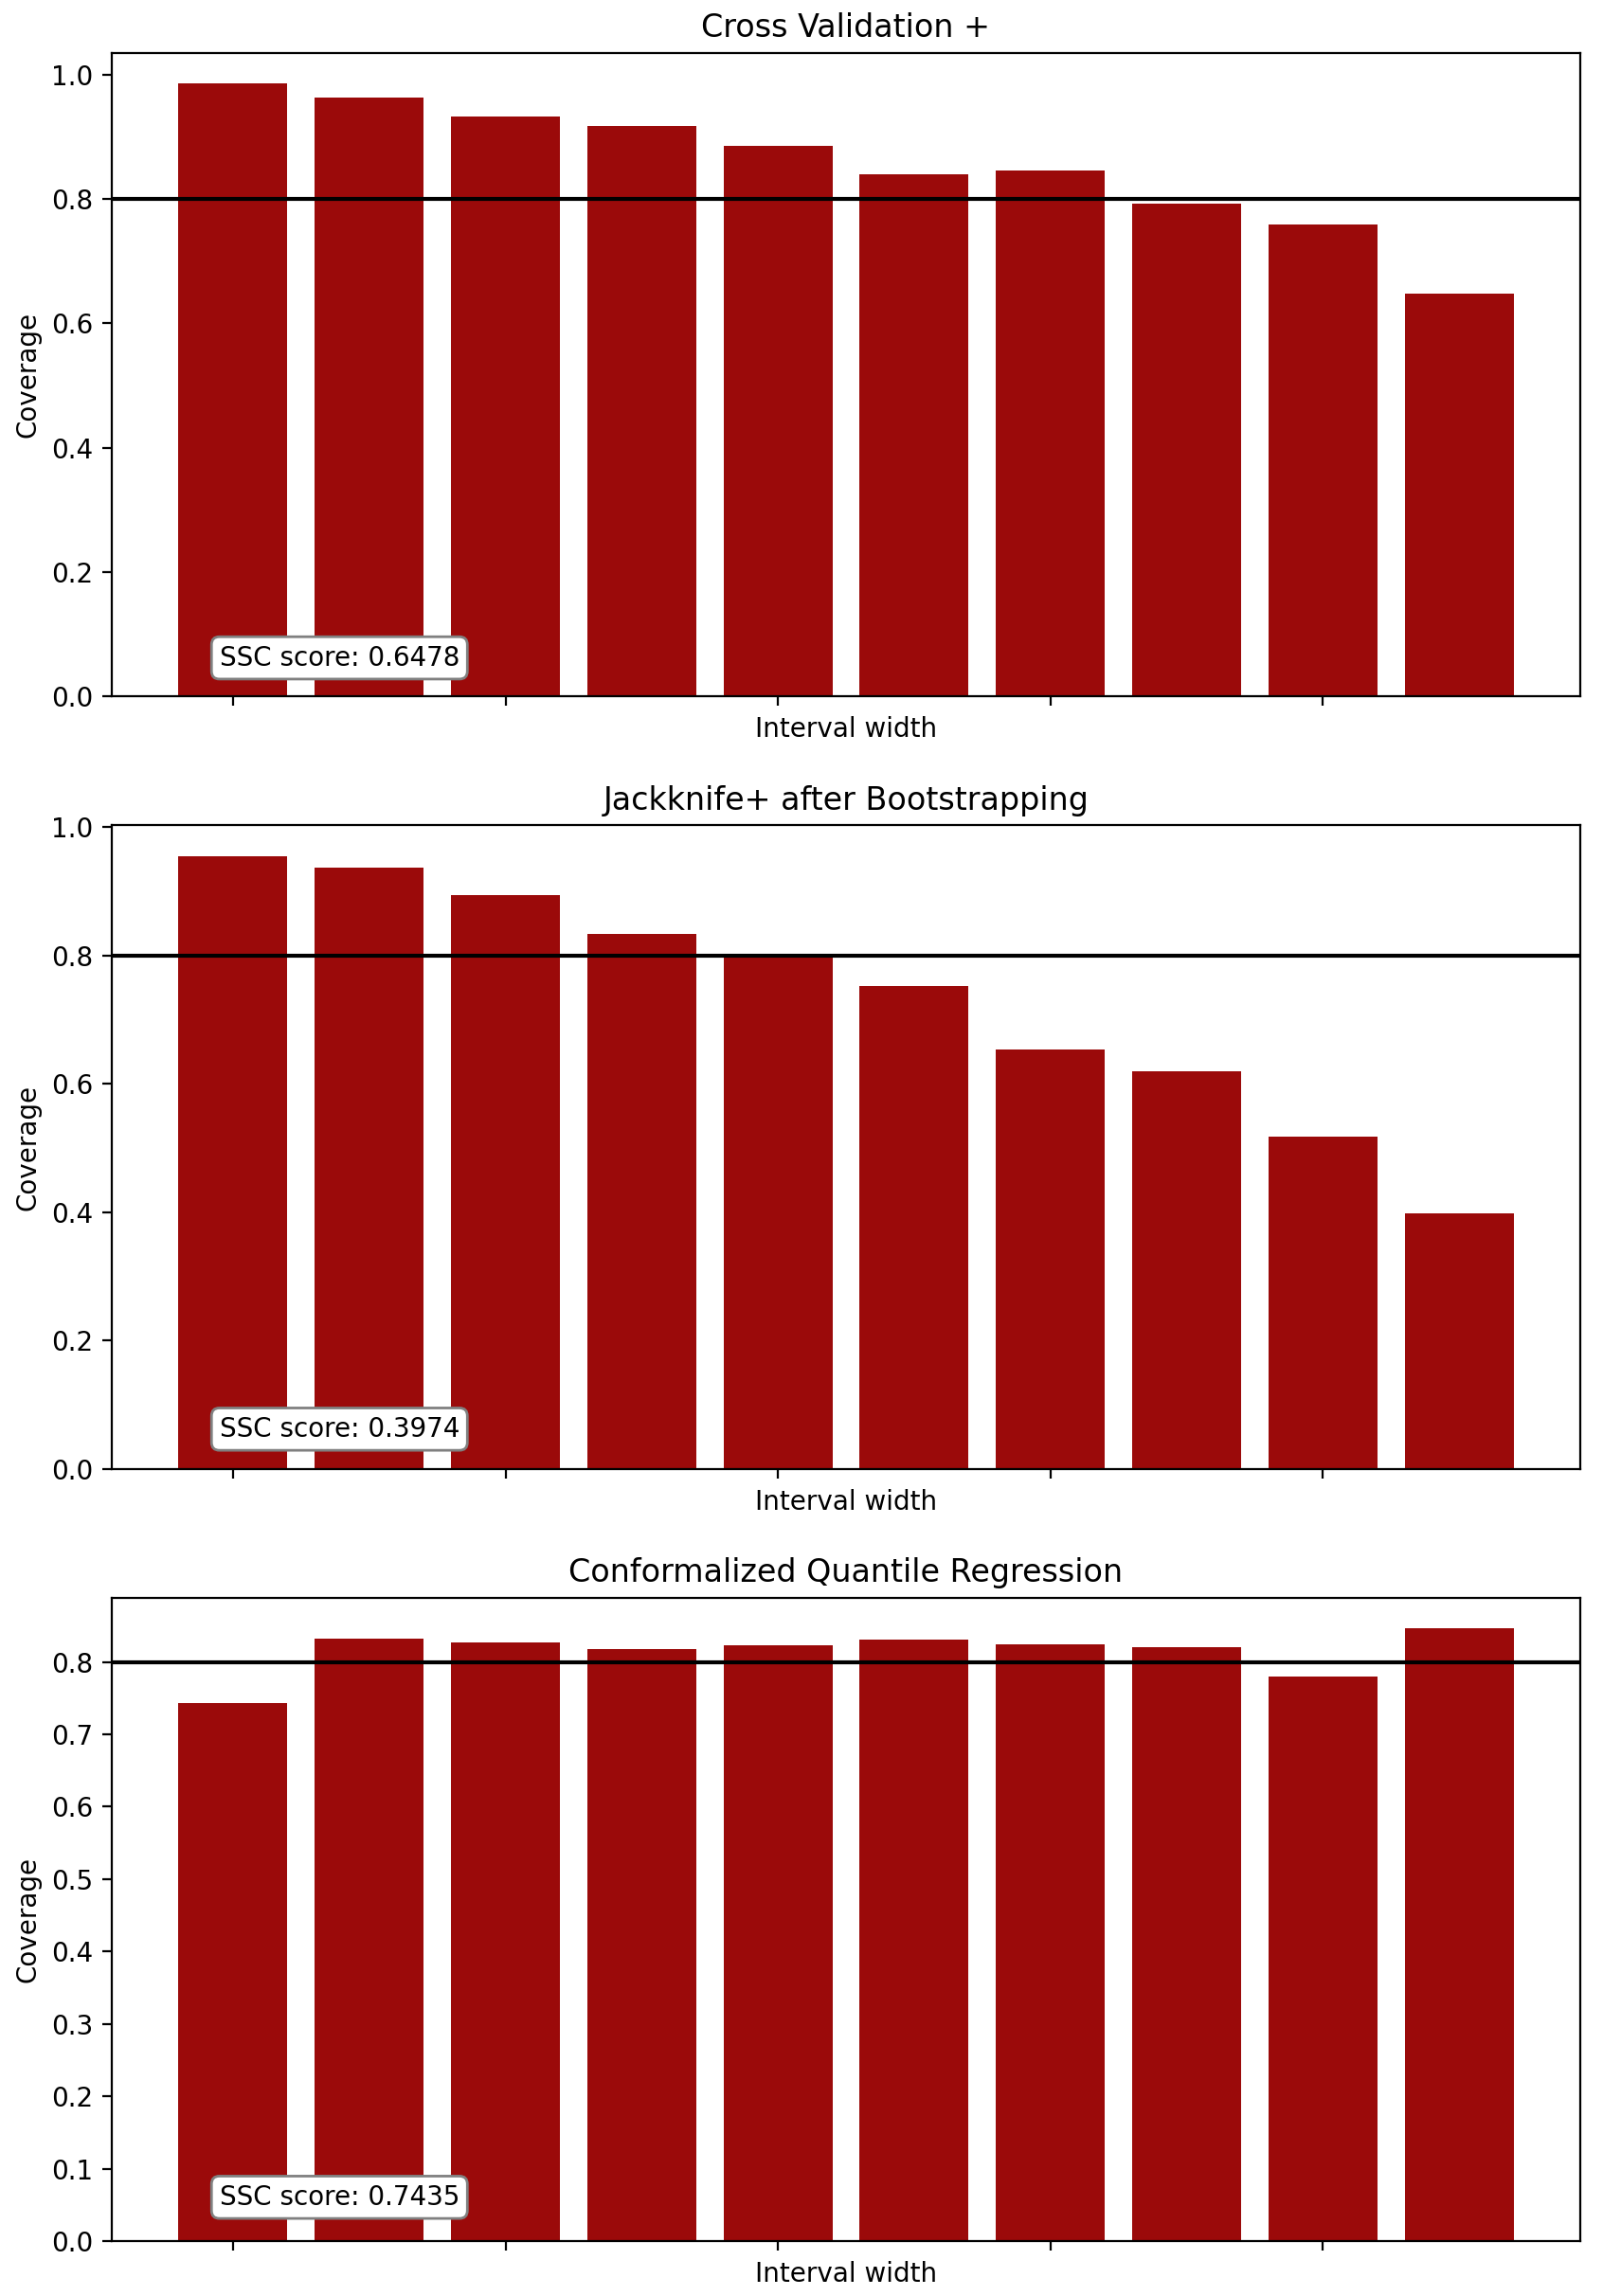
\includegraphics[width=1.15\textwidth, height=2.95\textwidth]{Figures/regression/coverage-vs-width-regression-problem.png}
        \caption{Coverage in function of intervals' width}
        \label{subfig:app-regression-coverage-width}
    \end{subfigure}
    \hfill % adds horizontal space between figures
    \begin{subfigure}[b]{0.32\textwidth} % Adjust the width to fit your needs
        \centering
        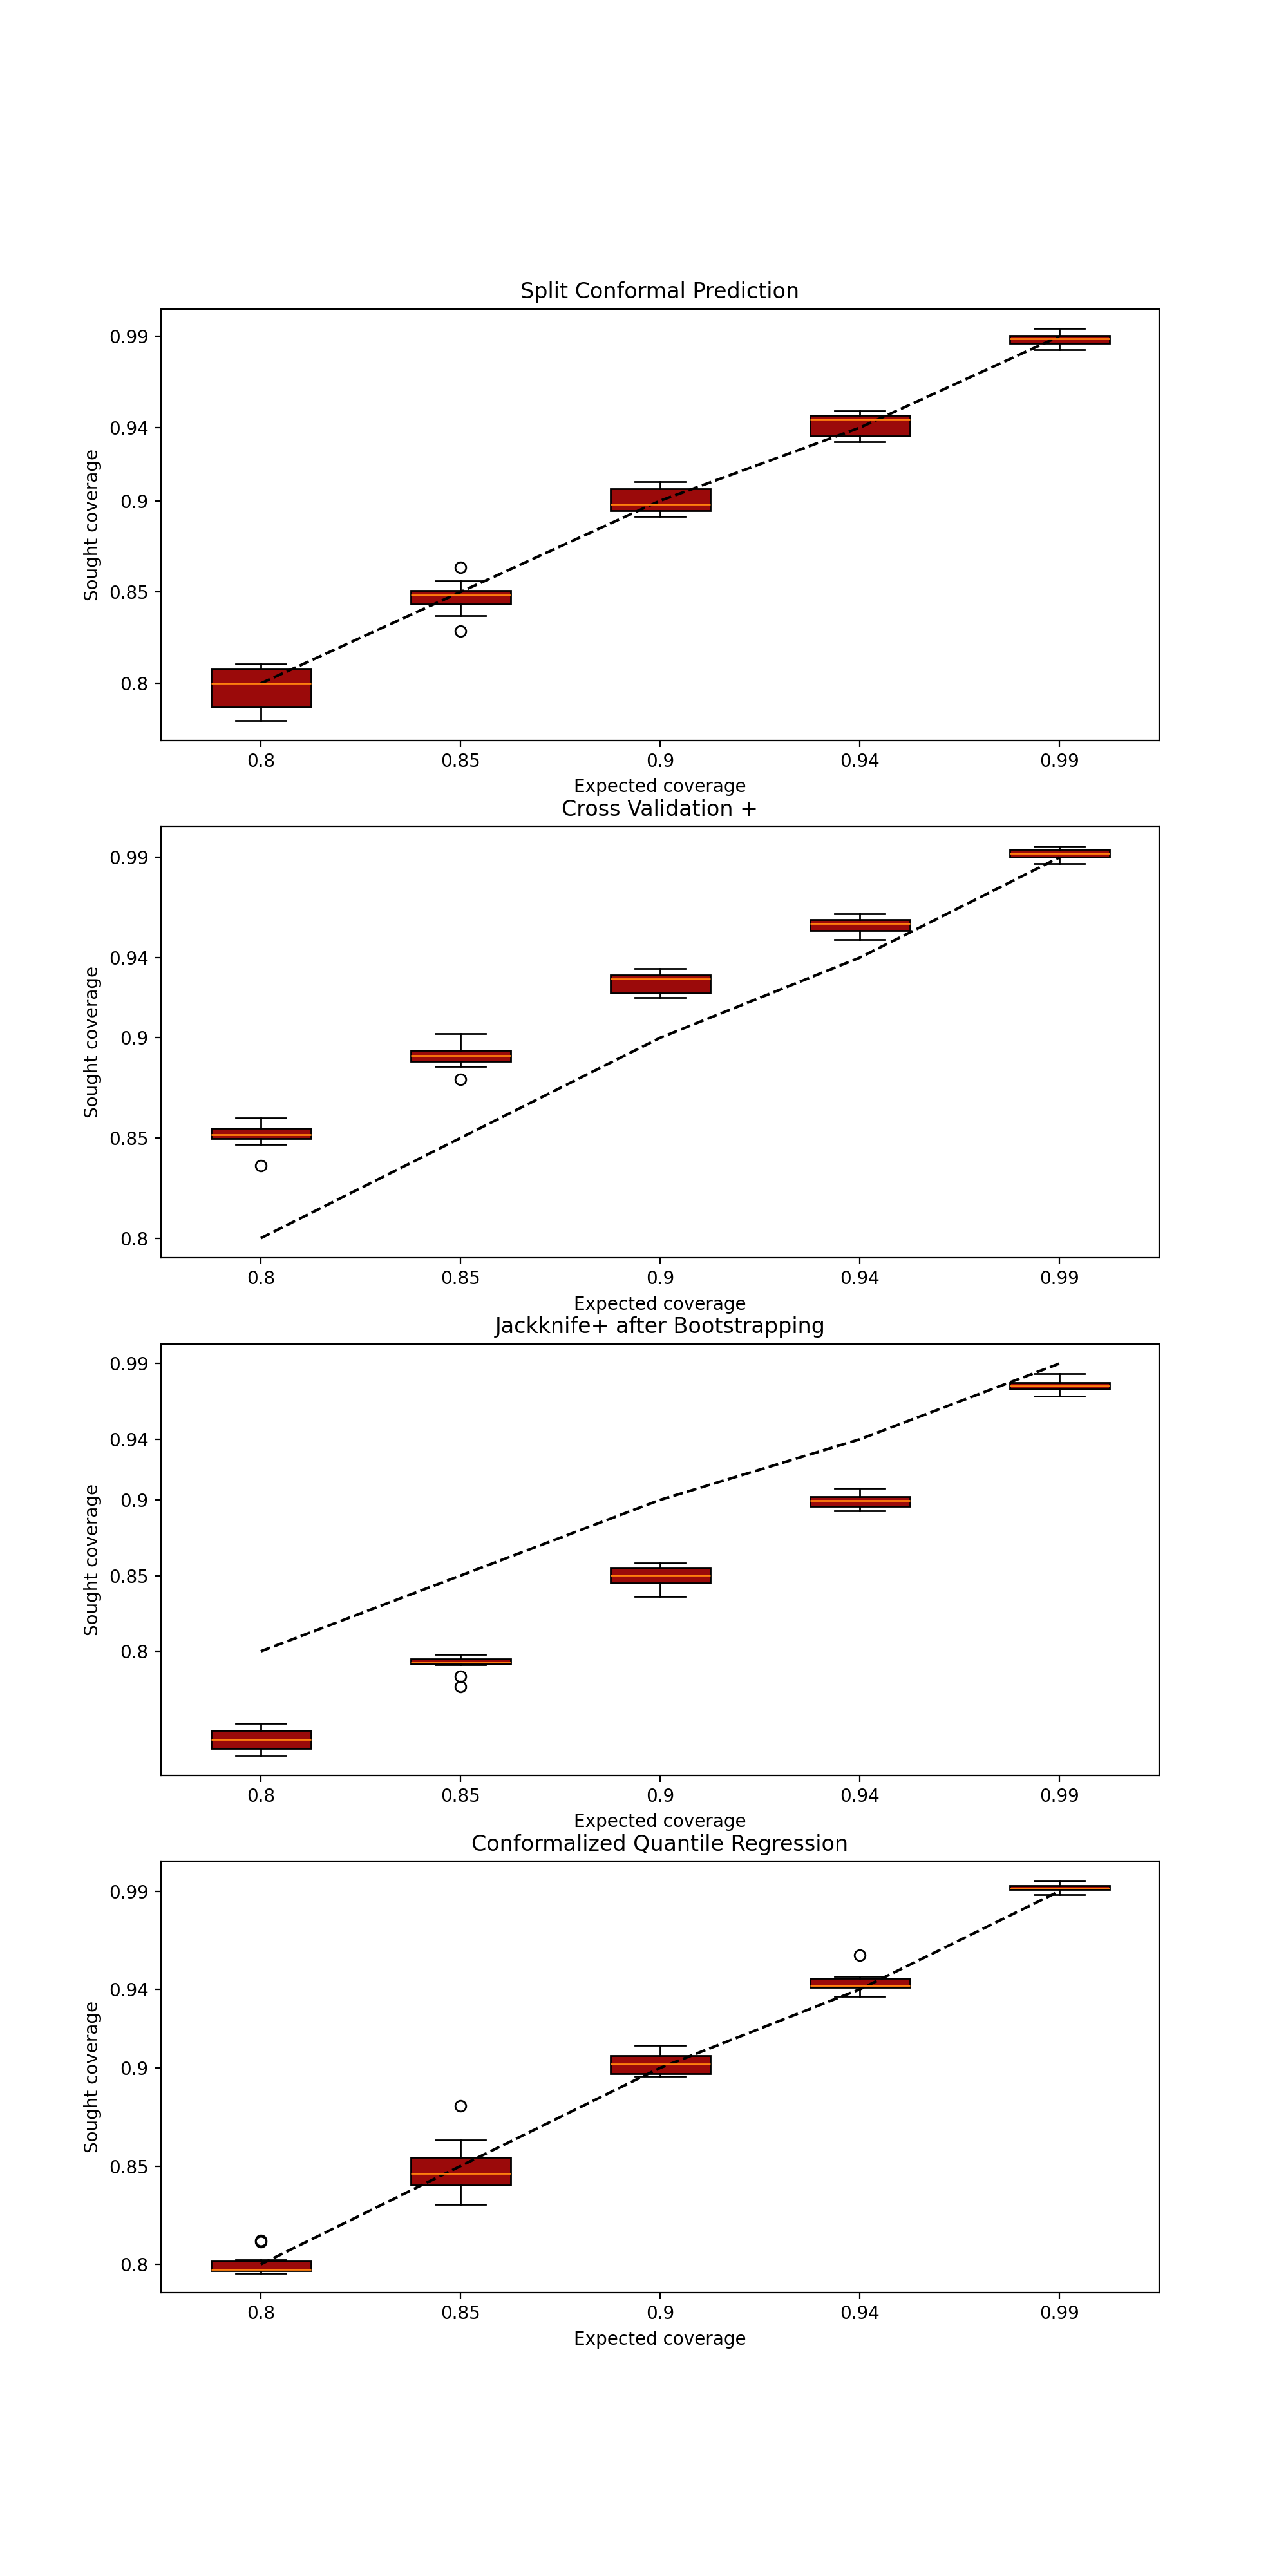
\includegraphics[width=1.15\textwidth, height=4\textwidth]{Figures/regression/coverage-vs-alpha-regression-problem.png} % Adjust the filename and path
        \caption{Coverage in function of $\a$}
        \label{subfig:app-regression-coverage-alpha}
    \end{subfigure}
    \caption{Visualizations related to width \& coverage distributions for the test data and 4 different strategies; from top to bottom: SCP, CV$+$, J$+$aB \& CQR. The first 2 plots just display the last 3 strategies, since SCP displays no adaptability at all (whereas J$+$aB slight to none adaptability).}
    \label{fig:app-regression-width-coverage}
\end{figure}

\begin{figure}[ht]
    \centering
    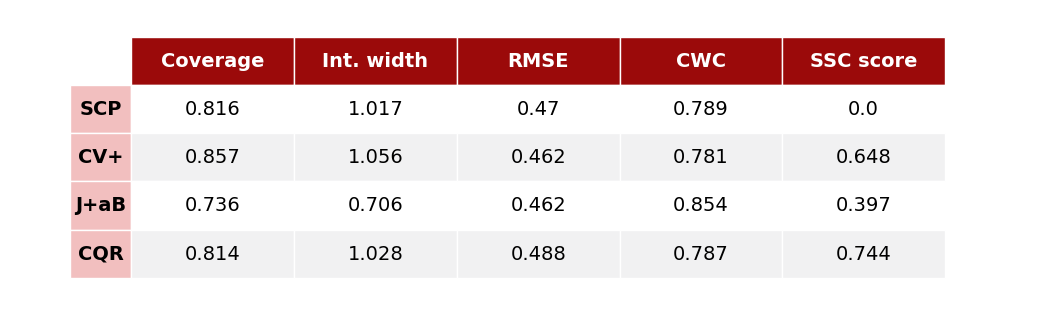
\includegraphics[width=\textwidth]{Figures/regression/metrics-table-regression-problem.png}
    \caption{Test data metrics for the 4 different strategies and 1 particular experiment (no 5-folds CV) for $\a=0.20$. From top to bottom: SCP, CV$+$, J$+$aB and CQR.}
    \label{fig:app-regression-metrics}
\end{figure}